\documentclass[12p,a4paper]{report}
\usepackage[utf8]{inputenc}
\usepackage[T1]{fontenc,url}
\usepackage{multicol}
\usepackage{multirow}
\usepackage{parskip}
\usepackage{lmodern}
\usepackage{microtype}
\usepackage{verbatim}
\usepackage{amsmath, amssymb}
\usepackage{tikz}
\usepackage{physics}
\usepackage{mathtools}
\usepackage{algorithm}
\usepackage{algpseudocode}
\usepackage{listings}
\usepackage{enumerate}
\usepackage{graphicx}
\usepackage{booktabs}
\usepackage{float}
\usepackage{hyperref}
\usepackage{tabularx}
\usepackage{siunitx}
\usepackage{fancyvrb}
\usepackage{blindtext}
\usepackage{tcolorbox}
\usepackage{relsize}
\usepackage{wrapfig}
\usepackage[explicit]{titlesec} %Control margins around titles.
\usepackage[makeroom]{cancel}
\usepackage[margin=1.2cm]{geometry}
\renewcommand{\baselinestretch}{1}
\renewcommand{\exp}{e^}
\renewcommand{\b}{\boldsymbol}
\newcommand{\h}{\hat}
\newcommand{\m}{\mathbb}
\newcommand{\half}{\frac{1}{2}}
\renewcommand{\exp}{e^}
\renewcommand{\bar}{\overline}
\newcommand{\lRightarrow}{\mathlarger{\mathlarger{\Rightarrow}}}
\setlength\parindent{0pt}


% Colorcoding. First for inside equations, second for text.
\definecolor{lightred}{RGB}{255,70,70}
\definecolor{lightgreen}{RGB}{140,255,140}
% Yellow
\newcommand{\yl}[1]{\colorbox{yellow}{$\displaystyle #1$}}
\newcommand{\yll}{\colorbox{yellow}}
% Green
\newcommand{\gr}[1]{\colorbox{lightgreen}{$\displaystyle #1$}}
\newcommand{\grr}{\colorbox{lightgreen}}
% Blue
\newcommand{\bl}[1]{\colorbox{cyan}{$\displaystyle #1$}}
\newcommand{\bll}{\colorbox{cyan}}
% Red
\newcommand{\rd}[1]{\colorbox{lightred}{$\displaystyle #1$}}
\newcommand{\rdd}{\colorbox{lightred}}

%\setlength{\tabcolsep}{6pt} % Default value: 6pt
%\renewcommand{\arraystretch}{1.5} % Default value: 1

%Options: Sonny, Lenny, Glenn, Conny, Rejne, Bjarne, Bjornstrup
%\usepackage[Bjornstrup]{fncychap}



\usepackage{eqparbox}   
\titleformat{\chapter}[block]{}{\eqmakebox[chap]{\Large\MakeUppercase{\sffamily\lsstyle\chaptername} %
\raisebox{-0.6\height}{\fontsize{50pt}{50pt}\selectfont\thechapter}\quad}}{0pt}{\huge\bfseries\raisebox{1ex}{\parbox[t]{\dimexpr\textwidth-\eqboxwidth{chap}\relax}{\titlerule[2pt]\vspace{1.25ex}#1}}}
\titlespacing*{\chapter}{0pt}{-32pt}{48pt}













\begin{document}


\setcounter{chapter}{3}
\chapter{Vector Spaces}
\section{Coordinate systems and mapping}
Consider a vector $\b x$ living in a vector space $V$. The vector $\b x$ is an abstract concept, living in some abstract space $V$. It may have some physical or gemoetric meaning or whatnot.

We now enforce a \textit{basis} onto $V$, called $\mathcal{B} = \{\b b_1,\dots, \b b_n\}$. This makes V \textit{behave like} $\m R^n$, in the sense that each vector $\b x$ in $V$ is \textit{mapped onto} a vector $[\b x]_\mathcal{B}$ in $\m R^n$. This is called a \textit{coordinate mapping} $\b x \mapsto [\b x]_\mathcal{B}$ "onto" the basis $\mathcal{B}$. The vector space $V$ might be foreign to us, and it can be important to create a mapping onto a more familiar vector space $\m R^n$, which we know how behaves. This transformation is "one-to-one", mapping each point in $V$ onto a point in $\m R^n$, and vice versa. This relation is called an \textbf{isomorphism}, and makes any vector space $V$ with a basis of $n$ vectors indistinguishable from $\m R^n$.

Usually, when a vector is written plainly as $\b x$, we consider it to be written in a \textit{standard basis} $\mathcal{E} = \{\b e_1,\, \b e_2\} = \begin{bmatrix} \,1\, \\ \,0\, \end{bmatrix},\, \begin{bmatrix} \,0\, \\ \,1\, \end{bmatrix}$, meaning that $\b x = [\b x]_\mathcal{E}$.

The relation between $\b x$ and $[\b x]_\mathcal{B}$ is given by a \textbf{change-of-basis matrix} $P_\mathcal{B}$, which consists of the basis-vectors of $\mathcal{B}$, written in the basis of $\mathcal{E}$:
\[
    \b x = P_\mathcal{B}[\b x]_\mathcal{B}  \quad\quad\quad  P_\mathcal{B} = [\b b_1\ \b b_2\ \dots\ \b b_n]
\]


\section{Change of basis}
This change of basis is just a special case of a more general change of basis between two basises $\mathcal{B} = \{\b b_1, \dots \b b_n\}$ and $\mathcal{C} = \{\b c_1, \dots \b c_n\}$, both spanning the same vector space $V$. The general change of basis is then
\[
    [\b x]_\mathcal{C} = \underset{\mathcal{C}\leftarrow\mathcal{B}}{P}\,[\b x]_\mathcal{B} \quad\quad\quad
    \underset{\mathcal{C}\leftarrow\mathcal{B}}{P} = \Big[[\b b_1]_\mathcal{C}\ [\b b_2]_\mathcal{C}\ \dots [\b b_1]_\mathcal{C}\Big]
\]

The change-of-basis matrix from $\mathcal{C}$ to $\mathcal{B}$ is simply the inverse: $\underset{\mathcal{B}\leftarrow\mathcal{C}}{P} = \qty(\underset{\mathcal{C}\leftarrow\mathcal{B}}{P})^{-1}$



\section{Linear transformations (mappings) between vector spaces}

\begin{wrapfigure}{r}{10cm}
    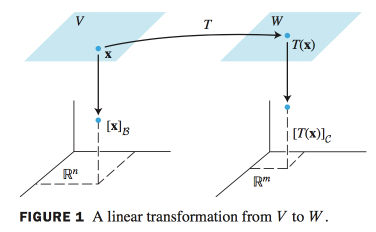
\includegraphics[width=8cm]{figs/map.jpg}
\end{wrapfigure} 
Consider two vector spaces $V$ and $W$, with basises $\mathcal{B} = \{\b b_1,\dots \b b_n\}$ and $\mathcal{C} = \{\b c_1,\dots, \b c_m\}$ in $\m R^n$ and $\m R^m$, respectively. We introduce a \textit{linear transformation} $T: V \mapsto W$ such that $T(\b x) = A\b x$. This is all well and good, but we might only have the vector $\b x$ represented in the basis $\mathcal{B}$, and usually want it written in the basis $\mathcal{C}$ after the transformation, as $\big[T(\b x)\big]_\mathcal{C}$.

What we want is some matrix $M$ that carries us straight from $[\b x]_\mathcal{B}$ to $\big[T(\b x)\big]_\mathcal{C}$. If we combine the change of basis with $T$, we get
\[
    \big[T(\b x)\big]_\mathcal{C} = M[\b x]_\mathcal{B}
\]
where
\[
    M = \Big[[T(\b b_1)]_\mathcal{C}\ \dots \ [T(\b b_n)]_\mathcal{C} \Big]
      = \Big[[A\b b_1]_\mathcal{C}\ \dots \ [A\b b_n]_\mathcal{C} \Big]
\]
This matrix is called the \textbf{matrix for T relative to the bases $\mathcal{B}$ and $\mathcal{C}$.}






\chapter{Eigenvalues and Eigenvectors}

If $A$ has $n$ independent eigenvalues, the eigenvectors of $A$ are linearly independent. If not, we don't know if they are linearly independent or not.


\section{Diagonalization}
If $A$ is a $n\times n$ matrix with with $n$ linearly independent eigenvectors $\b v_1, \dots, \b v_n$, with distinct eigenvalues $\lambda_1,\dots,\lambda_n$.


\chapter{asdf}
\chapter{Orthogonality and least squares}
\section{Projections}
\subsection{Projection of vector onto vector}
The projection of a vector $\b y$ onto another vector $\b x$ is
\begin{align*}
    \hat{\b y} = \frac{\b y \cdot \b x}{\b x \cdot \b x}\b x
\end{align*}



\subsection{Projection of vector onto subspace}
Let $W$ be subspace of $\m R^n$ with an orthogonal basis $\{\b u_1, \dots, \b u_p\}$ and $\b y$ be any vector in $\m R^n$. Then the projection of $\b y$ onto $W$ is simply the projection onto each basis-vector:
\begin{align*}
    \hat{\b y} = \frac{\b y \cdot \b u_1}{\b u_1 \cdot \b u_1}\b u_1 + \dots + \frac{\b y \cdot \b u_p}{\b u_p \cdot \b u_p}\b u_p
\end{align*}



\subsection{The Gram-Schmidt process of orthogonal factorization}
The Gram-Schmidt process takes any basis of vectors $\{\b x_1, \dots, \b x_p\}$ spanning a subspace in $\m R^n$, and creates a new \textit{orthogonal} basis of the same space, $\{\b v_1, \dots, \b v_p\}$.

The idea is to create one and one new vector $\b v_i$ from the corresponding $\b x_i$, \textit{but} subtract the projection of $\b x_i$ onto each of the former vectors $\b v_1, \dots, \b v_{i-1}$, such that the new vector is orthogonal to all formerly created vectors.
\begin{itemize}
    \item $\b v_1 = \b x_1$
    \item $\b v_2 = \b x_2 - \dfrac{\b x_2 \cdot \b v_1}{\b v_1 \cdot \b v_1}\b v_1$
    \item $\b v_3 = \b x_3 - \dfrac{\b x_3 \cdot \b v_1}{\b v_1 \cdot \b v_1}\b v_1
     - \dfrac{\b x_3 \cdot \b v_2}{\b v_2 \cdot \b v_2}\b v_2$
    \item \dots
\end{itemize}






\end{document}
